\documentclass{standalone}
\usepackage{graphicx}	
\usepackage{amssymb, amsmath}
\usepackage{color}

\usepackage{tikz}
\usetikzlibrary{intersections, backgrounds}
\usepackage{pgfmath}

\definecolor{light}{RGB}{220, 188, 188}
\definecolor{mid}{RGB}{185, 124, 124}
\definecolor{dark}{RGB}{143, 39, 39}
\definecolor{highlight}{RGB}{180, 31, 180}
\definecolor{gray10}{gray}{0.1}
\definecolor{gray20}{gray}{0.2}
\definecolor{gray30}{gray}{0.3}
\definecolor{gray40}{gray}{0.4}
\definecolor{gray60}{gray}{0.6}
\definecolor{gray70}{gray}{0.7}
\definecolor{gray80}{gray}{0.8}
\definecolor{gray90}{gray}{0.9}
\definecolor{gray95}{gray}{0.95}

\newcommand*{\offset}{0.025}

\begin{document}

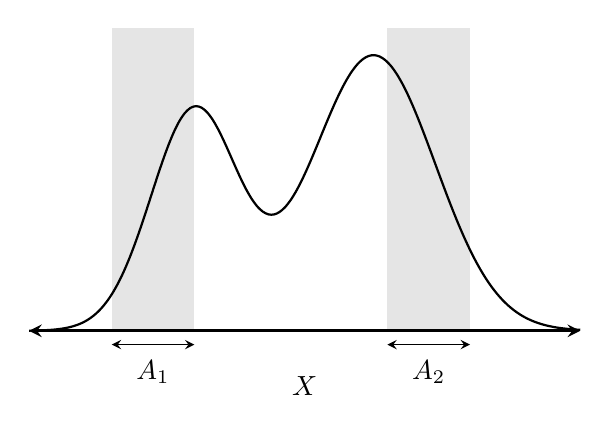
\begin{tikzpicture}[scale=0.35, thick, 
declare function={ g(\x) = 10 * exp(-0.1 * (\x - 2.5) * (\x - 2.5)) 
                          + 8 * exp(-0.2 * (\x + 4) * (\x + 4));},
]

  \fill[color=gray90] (-7, 0) rectangle (-4, 11);
  \draw [<->, >=stealth, line width=0.5] (-7, -0.5) -- (-4, -0.5);
  \node[] at (-5.5, -1.5) { $A_{1}$ };

  \fill[color=gray90] (3, 0) rectangle (6, 11);
  \draw [<->, >=stealth, line width=0.5] (3, -0.5) -- (6, -0.5);
  \node[] at (4.5, -1.5) { $A_{2}$ };

  \draw [<->, >=stealth, line width=1] (-10, 0) -- +(20, 0);
  \node[] at (0, -2) { $X$ };
  
  \draw[domain=-10:10, smooth, samples=100, variable=\x] 
    plot ({\x},{g(\x)});
   
\end{tikzpicture}

\end{document}  